\chapter{Implementação}

Após a apresentação do método, este capítulo tem por objetivo demonstrar a aplicação desta abordagem em diferentes exemplos. Para esta demonstração foram escolhidos cenários apresentados em trabalhos que SMA foram modelados de acordo com a organização $\mathcal{M}$oise$^{+}$. A escolha destes cenários se baseou na relevância dos autores, apresentarem a documentação das especificações necessárias para a aplicação do método e nível de complexidade.

\section{Writing paper}

\subsection{Descrição do cenário}

Este primeiro exemplo foi apresentado no trabalho \cite{kitio2008organisational} e estendido em \cite{hubner2011normative}, e representa um grupo de agentes com objetivo de escrever um artigo. A especificação estrutural desta organização descreve que ela é composta por apenas um grupo \textit{wpgroup} e este grupo possui dois papéis \textit{escritor} e \textit{editor} e ambos são sub-papéis de \textit{autor} Figura \ref{fig:writing-paper-estrutural}.
    
\begin{figure}[ht]
\centering
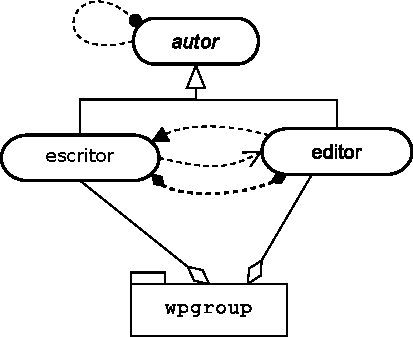
\includegraphics[scale=0.7]{imagens/5-writing-paper-estrutural.pdf}
\caption{Esquema social \textit{Writing paper}. Adaptado de \cite{hubner2011normative}}
\label{fig:writing-paper-estrutural}
\end{figure}
    
Para coordenar este grupo de agentes a atingir sua meta, um esquema funcional é definido Figura \ref{fig:writing-paper-funcional}. Neste esquema, primeiro um agente que assume a missão \textit{mMan} deve escrever uma versão de rascunho do artigo (\textit{fdv}), contendo como sub-metas escrever um título (\textit{wtitle}), um resumo (\textit{wabs}) e o título das seções (\textit{wsectitle}), sendo necessário atingir os objetivos nesta sequência. A segunda ramificação denominada \textit{sv}, versão de submissão é composta pelas metas \textit{wsec} escrever seção, e a finalização do artigo composta por duas metas em paralelo, escrever a conclusão \textit{wcon} e escrever as referências \textit{wref}.
    
\begin{figure}[ht]
\centering
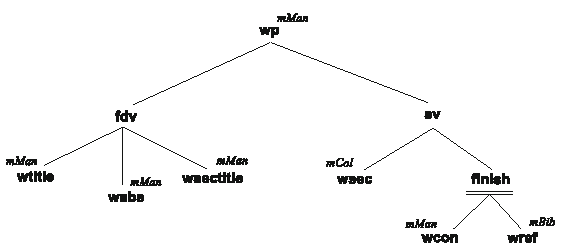
\includegraphics[scale=1.3]{imagens/5-writing-paper-funcional.pdf}
\caption{Especificação funcional \textit{Writing paper}. Adaptado de \cite{hubner2011normative}}
\label{fig:writing-paper-funcional}
\end{figure}

A Tabela \ref{tab:writing-paper-deontica} representa a especificação deôntica que define as permissões e obrigações dos papéis que assumem as missões. Estas missões são definidos por \textit{mMan} gerenciamento geral do projeto, composta por quatro metas, \textit{mCol} colaboração na escrita do conteúdo  e a missão \textit{mBib} em que o agente que assumir deverá reunir e escrever as referências do artigo.

\begin{table}[ht]
\centering
\caption{Especificação deôntica \textit{Writing paper}. \cite{hubner2011normative}}
\label{tab:writing-paper-deontica}
\begin{tabular}{@{}lll@{}}
\toprule
papel       & relação deôntica  & missão                        \\ \midrule
editor      & permissão         & \textit{mMan}                          \\
escritor    & obrigação         & \textit{mCol}                          \\
escritor    & obrigação         & \textit{mBib}                          \\
\bottomrule
\end{tabular}
\end{table}

\subsection{Implementação}

Seguindo a etapas do método, a ordem é:

\subsubsection{Declarações}

Baseado na especificação estrutural os papéis são editor e Escritor, com estas informações é possível codificar as \textit{Standard declaration} de acordo com o código abaixo.


\begin{lstlisting}
colset Role = with writer | editor | falha;
colset ROLES = list Role;
var w, e, f: ROLES;
\end{lstlisting}

\subsubsection{Estrutura}

A árvore de decomposição de metas do esquema social da Figura \ref{fig:writing-paper-funcional} é a base para a estrutura da RPC. Utilizando a relação dos operadores a estrutura da RPC é modelada de acordo com a Figura \ref{fig:5-estrutura1}.

\begin{figure}[ht]
\centering
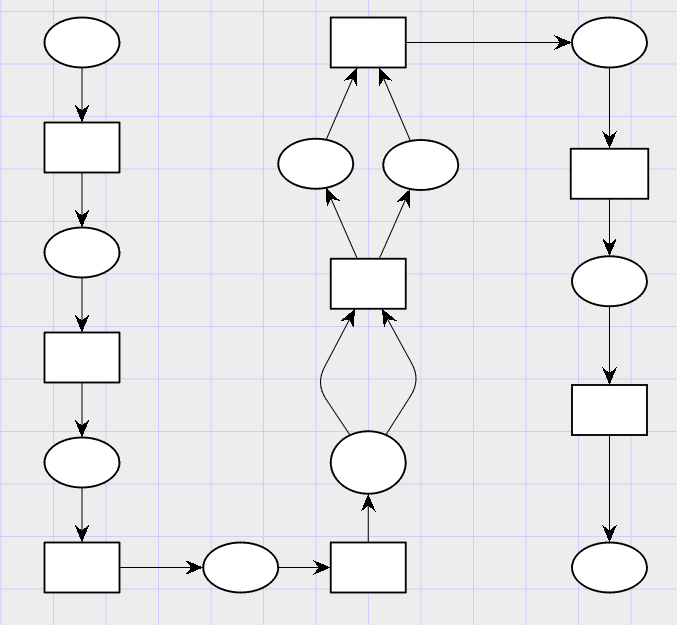
\includegraphics[scale=0.7]{imagens/5-estruturaRPC1.png}
\caption{Estrutura da RPC}
\label{fig:5-estrutura1}
\end{figure}

\subsubsection{Inscrições}

Através do esquema social e da especificação deôntica da Tabela \ref{tab:writing-paper-deontica} em que o papel editor é responsável pela missão \textit{mMan} e o papel escritor é responsável pelas missões \textit{mCol} e \textit{mBib} é possível determinar as inscrições da RPC. No nível folha em que um agente diferente começa uma missão deve conter uma ficha de inicialização neste lugar, para determinar que a transição seguinte tem como requisito a atuação do novo papel como pode ser visto na Figura \ref{fig:5inscricao1} no lugar \textit{wsec}.

\begin{figure}[ht]
\centering
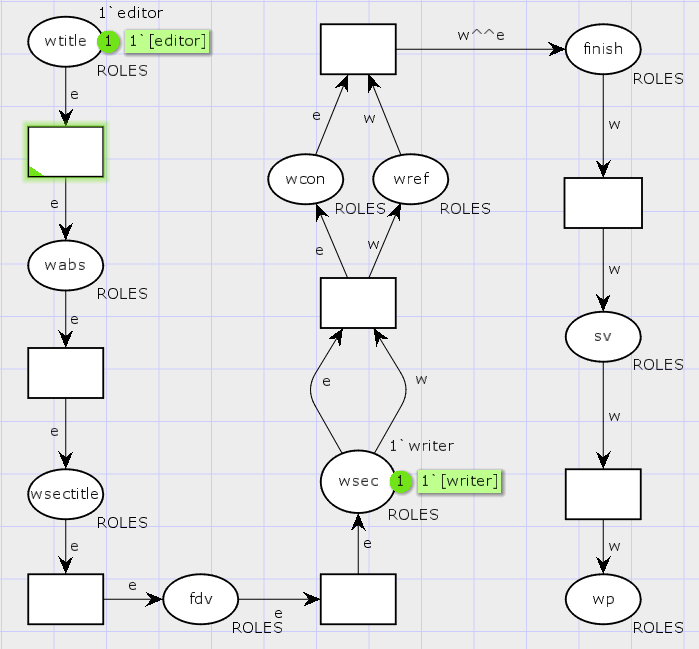
\includegraphics[scale=0.7]{imagens/5-inscricao1.png}
\caption{RPC com as inscrições.}
\label{fig:5inscricao1}
\end{figure}

\subsubsection{Falhas}

A etapa seguinte, inclusão das transições de falha, pode ser visto na Figura \ref{fig:5rpcfinal1}. Deve-se incluir uma transição, um lugar e uma transição auxiliar de falha para verificar se cada meta falhou, este processo é semelhante ao de \cite{winikoff2017bdi}, onde na Figura \ref{fig:control_fluxo} ele verificava se cada ação tinha falhado.

\begin{sidewaysfigure}[ht]
\centering
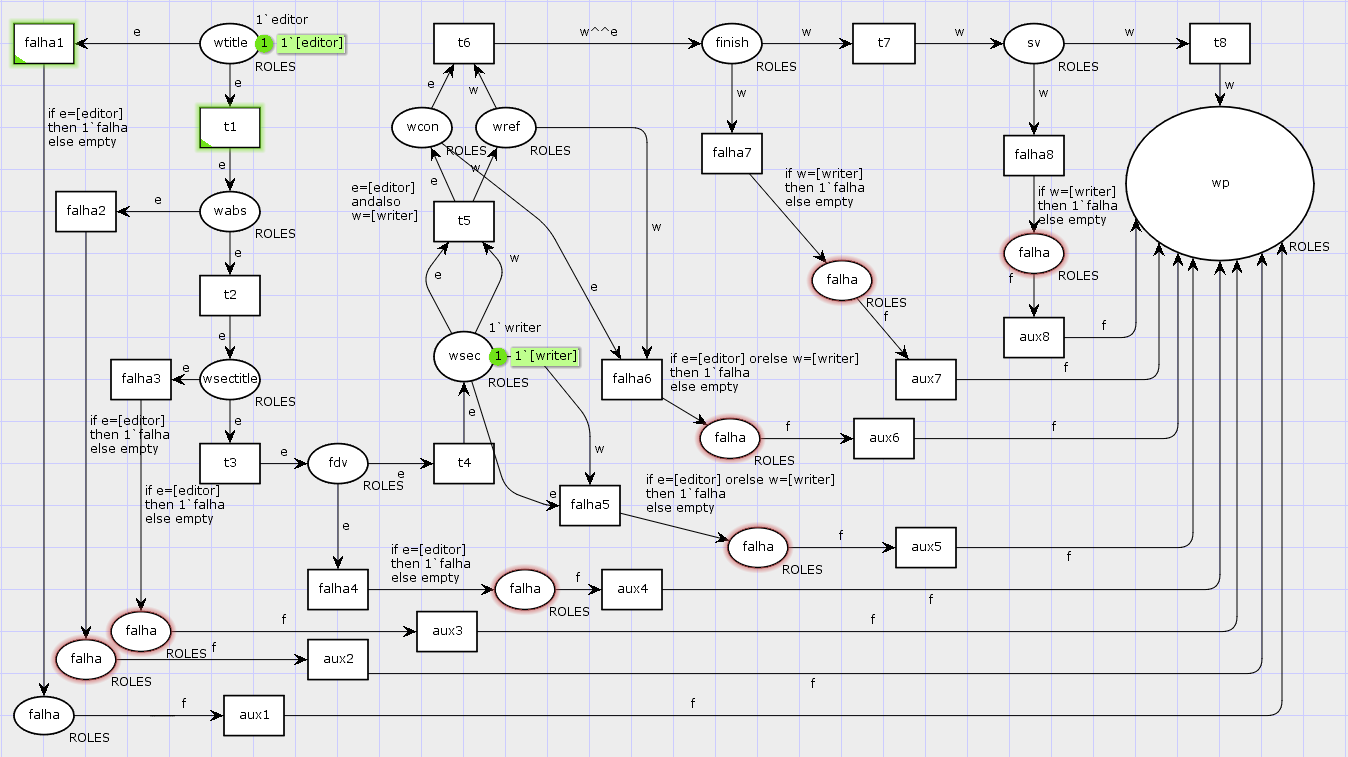
\includegraphics[scale=0.65]{imagens/5-implementacao1.png}
\caption{RPC com as transições de falha.}
\label{fig:5rpcfinal1}
\end{sidewaysfigure}

\subsubsection{Caminhos}

Para a avaliação de testabilidade do modelo, realizando a contagem de todos caminhos é necessário obter o arquivo gerado pelo CPN Tools ao salvar a RPC e inserí-lo na ferramenta. A ferramenta gera o grafo e apresenta como saída a contagem de todos os lugares, transições, arcos e caminhos, este último, o total de caminhos (Figura \ref{fig:5-resultado1}).

Os resultados número de caminhos, dezoito, números de transição, vinte e quatro e número de arcos, cinquenta e três são resultados da RPC e não do grafo. O resultado número de caminhos, representa o número de cenários de testes necessários para a cobertura do sistema.

\begin{figure}[ht]
\centering
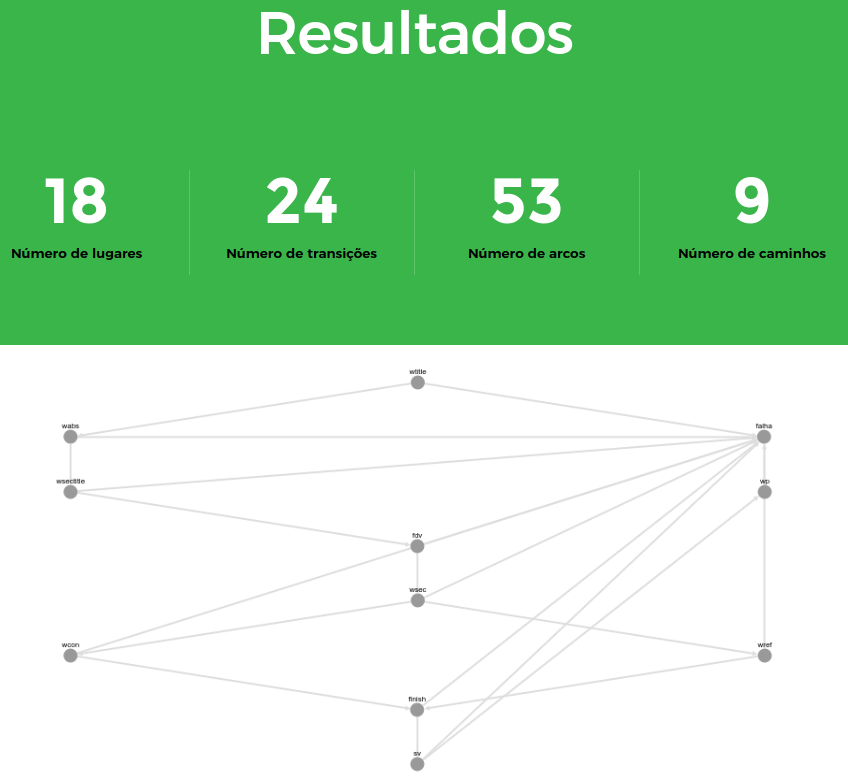
\includegraphics[scale=0.3]{imagens/5-resultado1.png}
\caption{Resultados da RPC \textit{Writing paper}.}
\label{fig:5-resultado1}
\end{figure}
    
\section{\textit{Multi-Agent Programming Contest- Agents on Mars}}

\subsection{Descrição do cenário}

Este cenário faz parte da \textit{Multi-Agent Programming Contest} \footnote[1]{https://multiagentcontest.org/}, um evento anual que tem o objetivo de estimular a pesquisa na área de desenvolvimento e programação de SMA. Através da competição, é possível avaliar e comparar diferentes aspectos dos sistemas desenvolvidos, identificando problemas, coletando \textit{benchmarks} e reunindo casos de teste que podem servir como referência para testar linguagens de programação multiagente, plataformas e ferramentas \cite{koster2012multi, ahlbrecht2013multi}.

Neste ano de 2013, o cenário da competição é Marte, onde os competidores deverão desenvolver agentes inteligentes autônomos para localizar poços de água, ocupar
as melhores zonas de Marte e sabotar seus rivais para conseguir seu objetivo ou para defender a si mesmos. Neste contexto, foi utilizado a solução da equipe SMADAS-UFSC que venceu a competição no ano de 2013 e desenvolveu a solução utilizando Jason, Cartago e $\mathcal{M}$oise$^{+}$ \cite{zatelli2013smadas, ahlbrecht2013multi}.

\begin{figure}[ht]
  \centering
  \subfigure[]{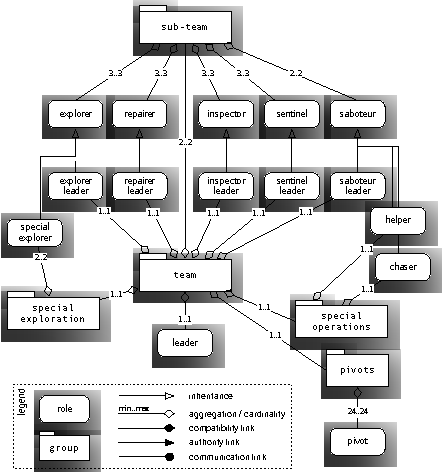
\includegraphics[width=0.45\textwidth]{imagens/marte-estrutural.pdf}\label{fig:marte-estrutural}}
  \subfigure[]{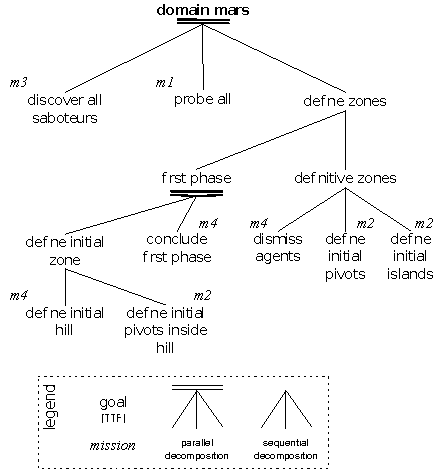
\includegraphics[width=0.45\textwidth]{imagens/marte-funcional.pdf}\label{fig:marte-funcional}}
  \caption{Agentes em Marte}
  \label{fig:marte}
\end{figure}


\begin{table}[ht]
\centering
\caption{Especificação deôntica \textit{Agentes em Marte}. \cite{zatelli2013smadas}}
\label{tab:marte-deontica}
\begin{tabular}{@{}llll@{}}
\toprule
norma   & papel         & relação deôntica  & missão                    \\ \midrule
n1      & explorer          & obrigação         & \textit{m1}               \\
n2      & sentinelLeader    & obrigação         & \textit{m2}               \\
n3      & inspector         & obrigação         & \textit{m3}               \\
n4      & explorerLeader    & obrigação         & \textit{m4}               \\
\bottomrule
\end{tabular}
\end{table}
  
\subsection{Implementação}

\subsubsection{Declaração}

Este exemplo como pode ser visto na Figura \ref{fig:marte-estrutural} possui mais papéis. Para esta modelagem, são declarados apenas os papéis utilizados na especificação social, e também presentes na especificação deôntica. A declaração encontra-se no código abaixo.

\begin{lstlisting}
colset Role = with explorer | sentinelLeader | inspector | explorerLeader | falha;
colset ROLES = list Role;
colset Sequence = product Role*Role;
var e, s, i, el, sl, seq: ROLES;
\end{lstlisting}

\subsubsection{Estrutura}

A criação de estrutura tem início pelo modo de leitura do esquema social, e obedecendo a relação entre operadores e as estruturas da RP. As metas \textit{discover all saboteurs}, \textit{probe all} e \textit{define zones} estão em paralelo, portanto elas são independentes para começar, mas a meta global \textit{domain mars} só poderá ser concluída quando todas as metas também estiverem concluídas. Logo, a estrutura da RPC para este modelo, foi definida na Figura \ref{fig:5-rpc-estrutura2}. O posicionamento dos lugares importa apenas para a RP ficar mais legível, o que determina por onde ela começa são as fichas, inscrições inseridas na próxima etapa.

\begin{figure}[ht]
\centering
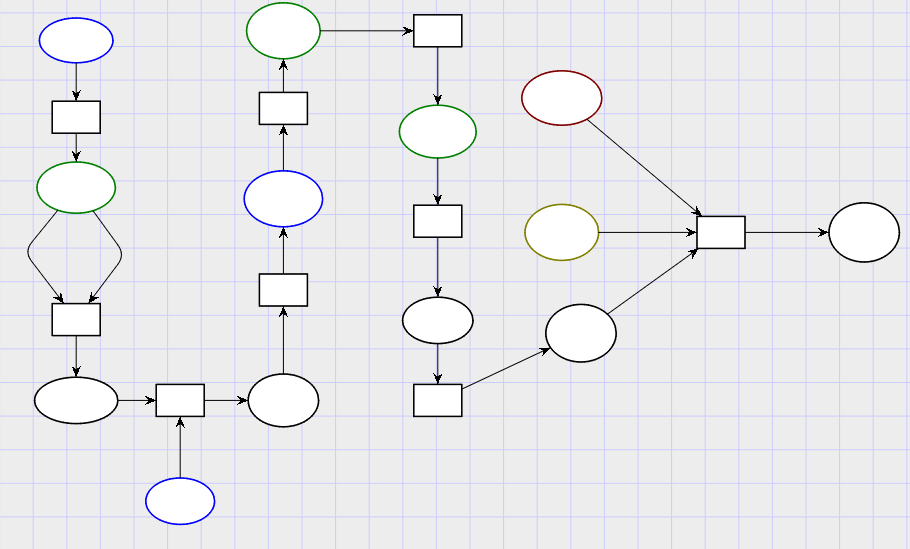
\includegraphics[scale=0.55]{imagens/5-rpc-estrutura2.png}
\caption{Estrutura da RPC \textit{Agents on Mars}.}
\label{fig:5-rpc-estrutura2}
\end{figure}

\subsubsection{Inscrições}

Na Figura \ref{fig:5-rpc-incricao} é possível ver as inscrições dos nomes dos lugares identificando as metas, as fichas identificando os papéis que atuam naquelas metas/lugares e também as inscrições nos arcos que determina que fichas são retiradas dos lugares iniciais e que fichas vão para o lugar final quando uma transição é disparada. As cores são apenas estilizações que podem ser utilizadas para identificar a que missão aquela meta/lugar está alocado.

Apesar dos lugares \textit{discover all saboteurs}, \textit{probe all} estaram no final da RP, é possível identificar pelas fichas que eles já estão prontos para serem disparados desde o início, tendo como dependência apenas a conclusão da meta \textit{define zones}. A dependência é criada na inscrição do arco de saída, exigindo que as três fichas estejam disponível para a transição ser disparada.

\begin{figure}[ht]
\centering
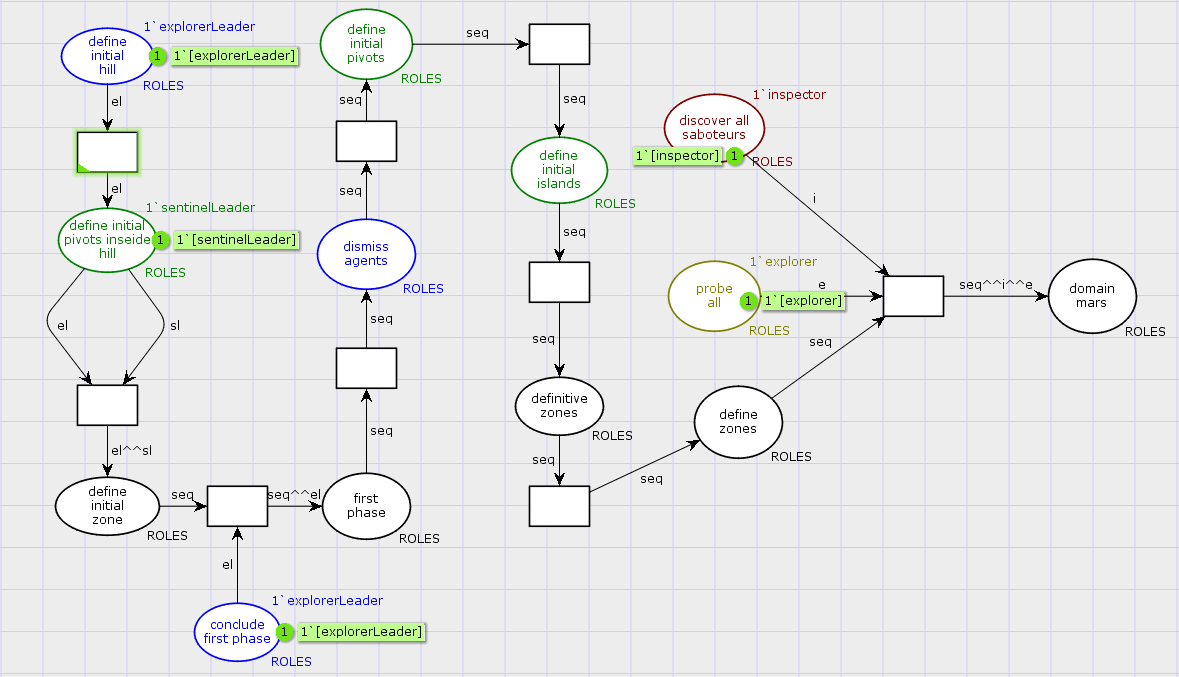
\includegraphics[scale=0.5]{imagens/5-rpc-incricao.png}
\caption{RPC \textit{Agents on Mars} com as inscrições.}
\label{fig:5-rpc-incricao}
\end{figure}

\subsubsection{Falha}

As transições de falha são inseridas obedecendo os operadores. Para uma melhor visualização elas são identificadas com a inscrição $ficha_{n}$. Elas recebem uma inscrição de arco que é uma função dependente da ficha recebida, caso a condição for verdadeira para a ficha o lugar final receberá uma ficha de falha, dependendo do modelo uma falha já poderá comprometer todo o sistema, caso não tenha nenhum laço de reparação. A Figura \ref{fig:5-rpc-final2} apresenta a RPC com as transições de falha.

\begin{sidewaysfigure}[ht]
\centering
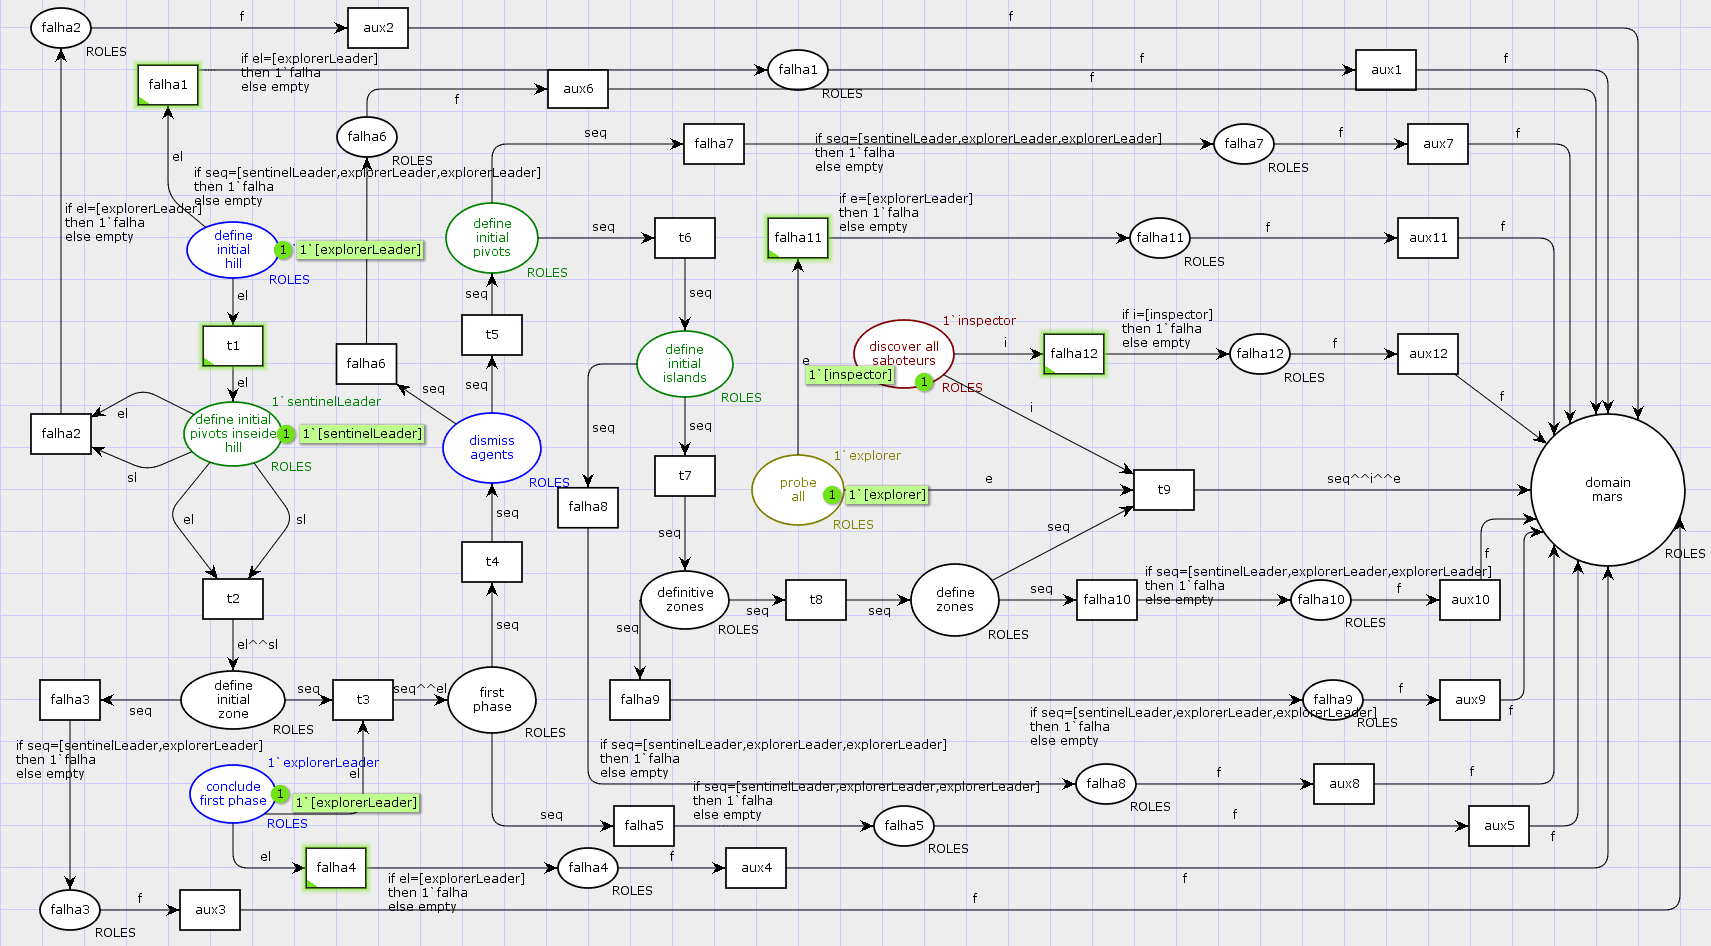
\includegraphics[scale=0.55]{imagens/5-implementacao2OK.png}
\caption{RPC \textit{Agents on Mars} com as transições de falha.}
\label{fig:5-rpc-final2}
\end{sidewaysfigure}

\subsubsection{Caminhos}
Nesta etapa, é necessário a inserção do arquivo gerado pela ferramenta CPN Tools ao salvar a rede, na ferramenta desenvolvida para a contagem de caminhos. O grafo gerado e os resultados são apresentados na Figura \ref{fig:5-resultado2}.

Entre os resultados são apresentadas as informações referente ao modelo de RPC, vinte e cinco lugares, trinta e três transições e 71 arcos. Estas informações podem ser utilizadas para comprar outros modelos para a mesma solução do problema. E o último resultado, número de caminho igual a treze, é o número de cenários de testes previstos para contemplar toda a cobertura do sistema.

\begin{figure}[ht]
\centering
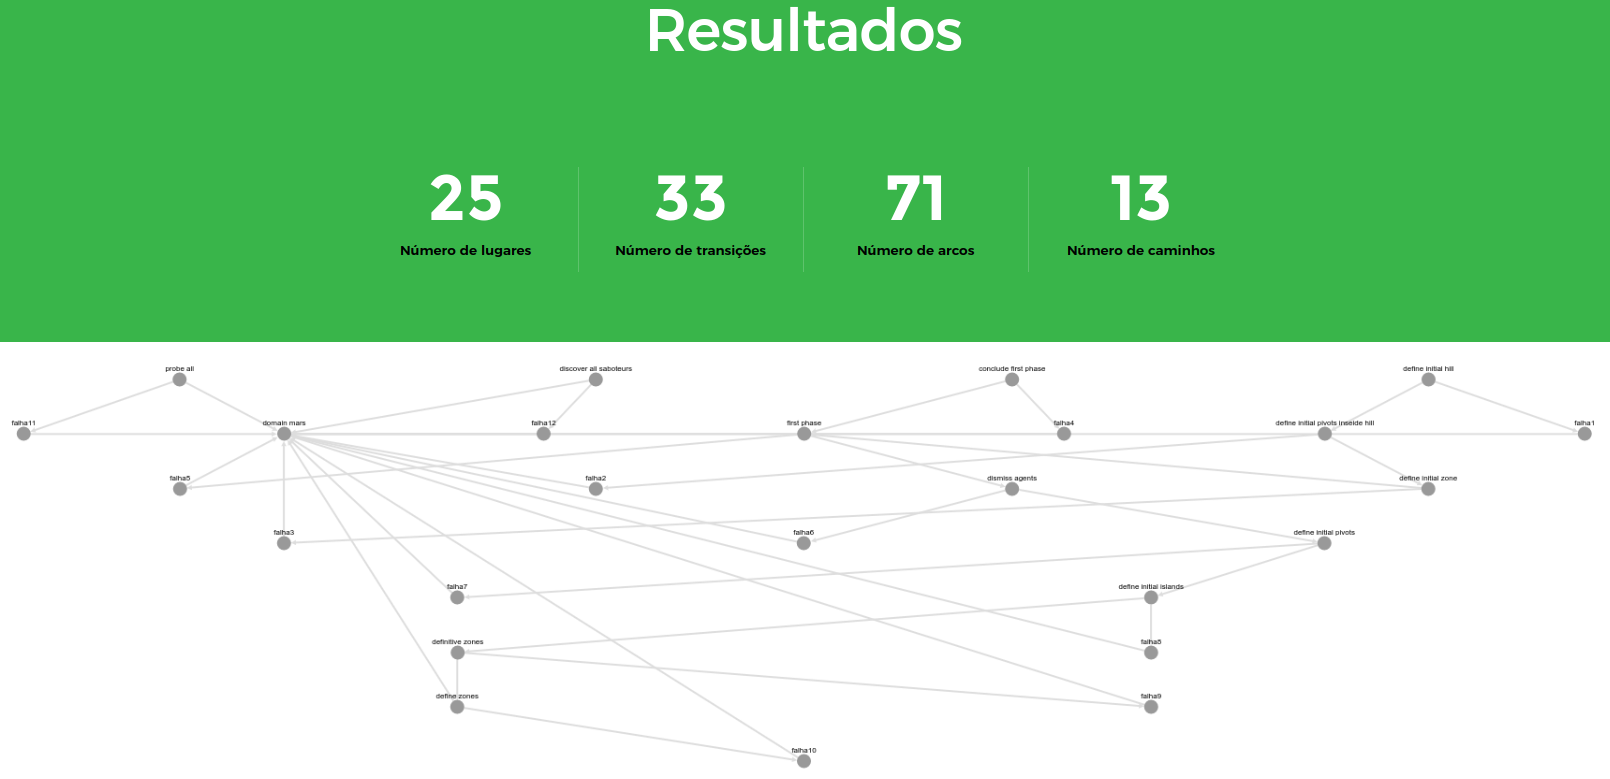
\includegraphics[scale=0.28]{imagens/5-resultado2.png}
\caption{Resultados da RPC \textit{Agents on Mars}.}
\label{fig:5-resultado2}
\end{figure}




\chapter{Conclusão}
Avaliar o número de casos de testes para softwares tradicionais com uma cobertura em um nível adequado não é uma tarefa fácil, avaliar este número de casos de testes com uma boa cobertura é ainda mais complicado devido a natureza autônoma dos agentes, que podem realizar seus objetivos de forma independente.

Esta dissertação propõem um método para a avaliação da testabilidade de SMA cuja organização é modelada através do $\mathcal{M}$oise. Este método permite modelar uma organização $\mathcal{M}$oise para uma RPC através de cinco etapas com os processos: declarações, estrutura, inscrições, falha e caminhos. Para avaliar a testabilidade contando os caminhos apresentados na RPC foi desenvolvido uma ferramenta que utiliza algoritmo de contagem de caminhos em grafos.

A principal contribuição deste trabalho é o método desenvolvido, que permite modelar em RPC sistemas multiagentes modelados pelo $\mathcal{M}$oise. Através das cinco etapas do processo e da  relação dos operadores da Figura \ref{fig:moise_rp} é possível modelar RPC que podem ser simuladas e avaliadas pelos recursos que as redes de petri oferecem. Uma contribuição secundária é uma ferramenta que realiza a contagem de caminhos de RP modeladas pela ferramenta CPN Tools, por padrão esta ferramenta não disponibiliza este tipo de análise.

Para os exemplos apresentados e modelados pelo método foi possível avaliar a testabilidade e obter números de cenários de testes necessários para a cobertura dos sistemas. Pela simplicidade dos exemplos, o número de cenários de teste é factível para realização dos testes, mas para exemplos mais complexos é possível que haja necessidade de escolha de áreas mais críticas do sistema para a criação de casos de uso focando por necessidade.

No entanto uma limitação apresentada pela pesquisa foi a modelagem das restrições de comunicação, característica do  $\mathcal{M}$oise$^{+}$ apresentada na especificação estrutural. Para incluir a modelagem de restrição de comunicação é necessário um nível onde os agentes estejam incluídos, assim permitindo uma simulação mais completa da RPC.

\section{Trabalhos Futuros}

Para um aperfeiçoamento e extensão do método além da correção da limitação descrita anteriormente são apontadas  possibilidades de trabalhos futuros.

\begin{itemize}
\item Extensão para o nível de agentes: para uma análise mais completa se um SMA, é necessário avaliar o comportamento dos agentes. Este comportamento poderia ser realizado utilizando ainda o $\mathcal{M}$oise$^{+}$ como modelo de organização e a base do método apresentada neste trabalho, mas utilizando em conjunto das RPC as RP Hierárquicas. Cada meta teria um subnível hierárquico que teria uma RP que faria a análise dos agentes e as ações que estes estão comprometidos.

\item Utilização do método em métodos de modelagem de sistemas orientados em agentes: Avaliar a utilização do método em métodos como o Prometheus ou outros que já provê diretrizes para o desenvolvimento de SMA.
\end{itemize}

